 \section{Методика исследования}

 \subsection{Использование информации о фактическом времени ответа}

Выражение для прогнозного времени ответа можно использовать для вы\-явления абер\-раций (отклонений) в поведении пользователя (см. \cite{6.}). Для этого введём понятие отклонения (ошибки) прогноза.

Отклонением прогноза будем разность между прогнозным временем ответа и фактичес\-ким временем ответа студента. В логарифмической шкале разность будет иметь вид отноше\-ния
\begin{equation}
E_{ij} = \ln \tilde{T}_{ij} - \ln t_{ij} =  \ln \frac{\tilde{T}_{ij}}{t_{ij}}
\end{equation}

Из этого отношения можно сделать вывод, что ошибка прогноза - случайная величина, которая имеет нормальное распределение c параметрами
\begin{equation}
\label{resudal}
E_{ij} \sim N\left(\mu + \beta_i + \tau_j - \ln t_{ij},\sigma^{2}_{ij}\right).
\end{equation}

Таким образом, выявление отклонений в поведении студента сводится к задаче проверки того факта, что реализации $e_{ij}$ случайной величины $E_{ij}$ имеют нормаль\-ное распределение с соответствующими параметрами, инди\-видуальными для каждого студента и каждой задачи. Алгоритм такой про\-верки будет описан ниже.

\subsection{Обработка экспериментальных данных}

Для применения на практике теоретических положений и математичес\-ких моделей, описанных в разделе \ref{ch22}, исследовались реальные данные пользова\-телей системы дистанцион\-ного обучения МАИ. На момент написания диплома в системе не фиксировалось время, которое студент тратит на решение конт\-рольных и тестовых задач. В связи с этим в исходный код системы дистан\-ционного обучения и структуру базы данных, которая исполь\-зуется системой, были внесены доработки, позволяющие фикси\-ровать время ответа для всех существующих курсов (<<Математический ана\-лиз>>, <<Линейная алгебра и ана\-литическая геометрия>>, <<Теория вероятностей и математическая статистика>>).

После внесённых изменений система фиксирует следующие данные: сколь\-ко раз была отображена каждая задача, сколько попыток произвел каждый студент для её решения и какое количество времени было затрачено для каждой из попыток. Таким образом, мы получаем набор исходных данных для статистической обработки в виде базы данных MySQL

Для получения оценок параметров модели, описанных в разделе \ref{oppmpv}, обра\-ботаем полученную статистику. Порядок обработки статистики покажем на примере задачи № 8.2.3 из курса <<Математический анализ>>

Вначале построим гистограмму для времени, которое студенты затра\-чивали для ответа на задачу
\begin{figure}[ht!]
\centering 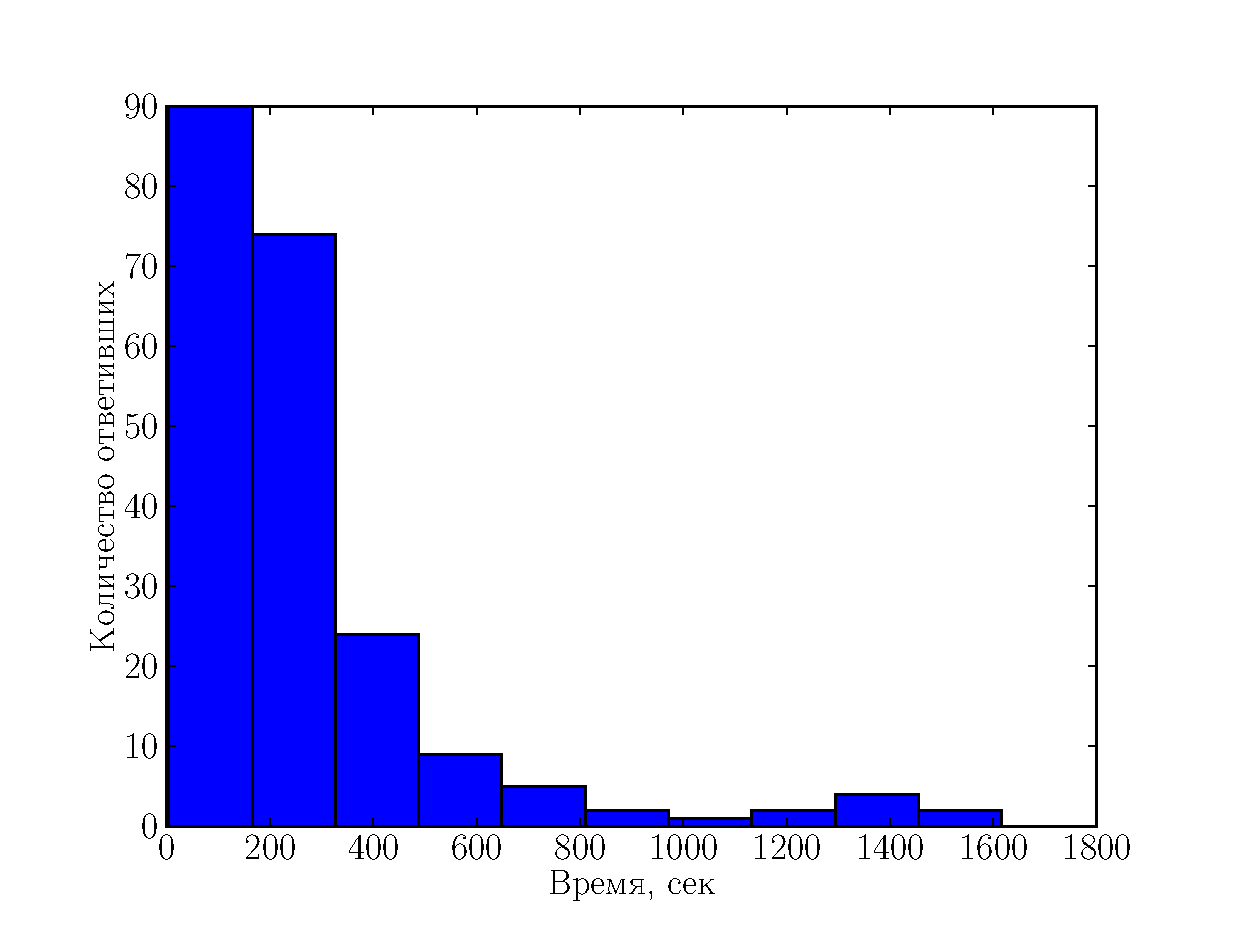
\includegraphics[scale=0.6]{test.eps}
\caption{Гистограмма времени ответа}
\end{figure}


Согласно модели, построенной в разделе \ref{mvonu}, применим логарифми\-ческое преобразование к времени ответа и построим гистограмму полученных значений:
\begin{figure}[ht!]
\centering 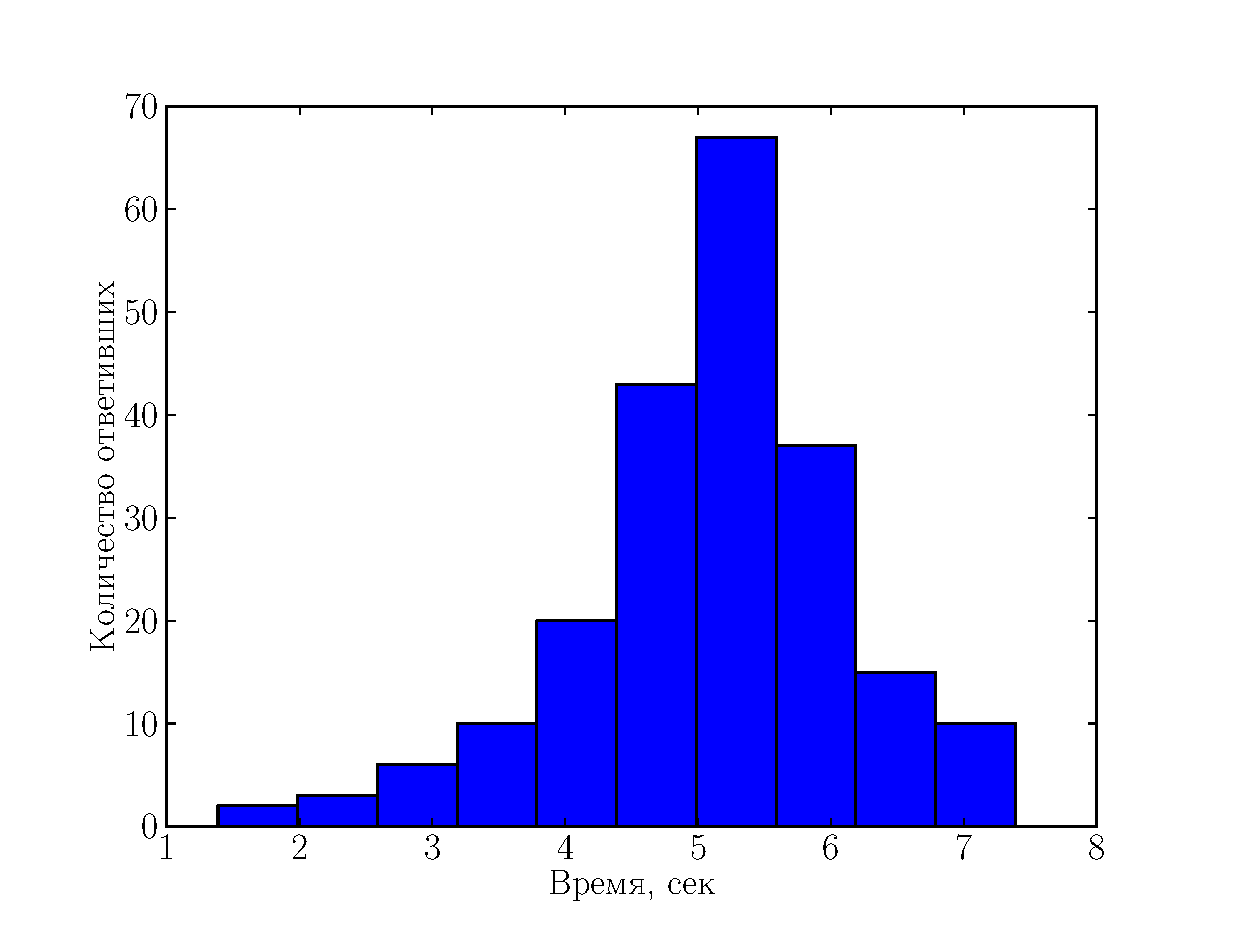
\includegraphics[scale=0.6]{test1.eps}
\caption{Гистограмма времени ответа (логарифмический масштаб)}
\end{figure}

Как видно из данного примера, применение логарифмического преобра\-зования к выборке по времени ответа обучающихся позволяет получить сим\-метричный вид распределения, который походит на нормальное распреде\-ление. 

Проверим статистическую гипотезу о нормальности распределения, ис\-пользуя критерий, основанный на понятиях ассиметрии и эксцесса (см. \cite{11.,12.}). Выбор критерия обусловлен скоростью его работы (т.к. необходимо обра\-батывать большое количество выборок объёма $n\ge20$). Выборочные оценки параметров асиметрии и эксцесса для выборки объёма $n$ имеют вид:
$$
\alpha_3 = \frac{1}{ns^3}\sum\limits_{i=1}^{n}(x_i-\overline{x})^3 - \mbox{ асимметрия};\; \alpha_4 = \frac{1}{ns^4}\sum\limits_{i=1}^{n}(x_i-\overline{x})^4 - \mbox{ эксцесс},
$$
где $s^2 = \frac{1}{n}\sum\limits_{i=1}^{n}(x_i-\overline{x})^2$ - выборочная дисперсия. Для выборки, которая пред\-ставляет собой реализации нормально распределённой случайной величины, моменты принимают значения $\alpha_3=0$ и $\alpha_4 = 3$.

Для проверки гипотезы о нормальном распределении мы будем исполь\-зовать комбинированный $K^2$-критерий (см. \cite{13.}). Статистика критерия имеет вид:
$$
K^2 = X^2(\alpha_3) + X^2(\alpha_4),
$$
где $X(\alpha_3), X(\alpha_4)$ - стандартная нормальная аппроксимация $\alpha_3$ и $\alpha_4$\cite{37.}.

Если основная гипотеза является истинной, статистика $K^2$ имеет распре\-деление $\chi^2$ с $f=2$ степенями свободы. Критическая область для значения статистики $K^2$ на выборке $X$ для уровня значимости $\alpha$ имеет вид $K^{2}_{X} > \chi^{2}_{1-\alpha}(2)$. Тест проводился на выборках размером $s>20$ для использования стандартной нормальной аппроксимации. В таблице приведены значения объ\-ёма выборки $n$ , ассиметрии $\alpha_3$ , эксцесса $\alpha_4$, статистики $K^2$. Значение кван\-тили для уровня значимости $\alpha = 0.05$ составляет $\chi^{2}_{0.95}(2) = 5.99$ (критическая точка). Критическая область находится справа от критической точки, т.е. если значение статистки больше $5.99$ - гипотеза о нормальности распределе\-ния отклоняется на уровне значимости $0.05$.


\begin{table}[H]
\caption{Проверка гипотезы о нормальном распределении}
\label{tabular:IRTtable}
\begin{center}
\begin{tabular}{|c|c|c|c|c|}
\hline
%Задача & $\chi^2$ & p-value\\
Задача & $n$   & $\alpha_3$ & $\alpha_4$ &$K^2$\\
\hline
1.2.5 & 31 & -0.08 & 2.53 & 0.11 \\ 
\hline
1.2.8 & 25 & 0.05 & 2.95 & 0.256 \\ 
\hline
10.3.2 & 21 & -0.18 & 2.85 & 0.329 \\ 
\hline
11.2.4 & 51 & -0.12 & 2.78 & 0.144 \\ 
\hline
2.2.2 & 42 & -0.14 & 2.5 & 0.41 \\ 
\hline
2.2.7 & 58 & 0.18 & 2.89 & 0.417 \\ 
\hline
4.2.1 & 48 & -0.08 & 2.67 & 0.094 \\ 
\hline
5.3.4 & 21 & 0.11 & 2.59 & 0.066 \\ 
\hline
6.1.3 & 41 & -0.14 & 2.6 & 0.23 \\ 
\hline
6.2.5 & 90 & -0.09 & 2.92 & 0.178 \\ 
\hline
6.3.10 & 25 & 0.24 & 2.54 & 0.366 \\ 
\hline
6.3.2 & 29 & -0.2 & 2.95 & 0.487 \\ 
\hline
6.3.4 & 27 & -0.07 & 2.42 & 0.193 \\ 
\hline
7.2.7 & 73 & -0.0 & 2.8 & 0.002 \\ 
\hline
7.3.1 & 32 & -0.04 & 2.49 & 0.142 \\ 
\hline
7.3.6 & 31 & -0.23 & 2.51 & 0.465 \\ 
\hline
\end{tabular}
\end{center}
\end{table}

Из таблицы видно, что вычисленнные значения статистики попадают в доверительную область критерия. Таким образом, время ответа на задачу в СДО имеет нормальное распределение.

Приведём оценки для параметров модели. Модель, описанная уравнением (\ref{mainmodel}) применяется к экспериментальным данным следующим образом: пусть для каждого студента $j$ из общего количества студентов $M$ система дистан\-ционного обучения случайным образом выбирает $k$ задач из пула задач объ\-ёма $K$. Тогда по результатам тестирования мы получаем следующую таблицу:
\begin{table}[H]
\caption{Время ответа}
\label{tabular:IRTtable}
\begin{center}
\begin{tabular}{|c|c|c|c|c|}
\hline
 & \multicolumn{4}{|c|}{Студент}\\
 \hline
 Задача & 1 & 2 & \dots & M \\
 \hline
 1 & $t_{11}$ & $t_{12}$ & \dots & $t_{1M}$\\
\hline
 2 & $t_{21}$ & $t_{22}$ & \dots & $t_{2M}$\\
\hline
 \vdots & \vdots & \vdots & \vdots & \vdots\\
\hline
 K & $t_{k1}$ & $t_{k2}$ & \dots & $t_{kM}$\\
\hline
\end{tabular}
\end{center}
\end{table}

Таблица отражает время $t_{ji}$, которое затратил студент  $j$ при ответе на задачу $i$. Время ответа имеет логнормальное распределение, согласно п. (\ref{mainmodel}).

Оценка параметров модели происходит на основании данных таблицы (\ref{tabular:IRTtable}) согласно формулам (\ref{1166}) - (\ref{1167}). Операции по индексу $i$ представляют с собой операции над строками таблицы, операции по индексу $j$ -  над столбцами. Приведём оценки параметров для группы из случайным образом выбранных $M=15$ студентов, которые проходят тест из $k=16$ задач.

Параметры студентов:
\begin{table}[H]
\caption{Параметры студента}
\label{tabular:IRTtable}
\begin{center}
\begin{tabular}
{|c	|c	|c	|c	|c	|c	|c	|c	|c	|c	|c|}
\hline
id студента  		&	400			&	450		&	243		&	198			&	534			&	\ldots			&	537		&	652		&	126		&	158	\\ 
\hline
$\tau$ студента		&	-0.37		&	1.4		&	-0.69	&	-0.73		&	-0.13		&	\ldots		&	-0.17		&	-0.04		&	1.51		&	1.32	\\
\hline
\end{tabular}
\end{center}
\end{table}

Параметры задач:
\begin{table}[H]
\caption{Параметры задачи}
\label{tabular:IRTtable}
\begin{center}
\begin{tabular}
{|c	|c	|c	|c	|c	|c	|c	|c	|c	|c|}
\hline
задача  		&	10.3.2		&	6.3.4		&	11.2.4		&	1.2.5		&	\ldots		&	6.1.3		&	7.3.1		&	4.2.1		&	1.2.8	\\ 
\hline
$\beta$ задачи	&	1.47		&	1.08		&	-0.75		&	-1.17		&	\ldots		&	0.94		&	1.5		&	-0.6		&	-0.85	\\
\hline
\end{tabular}
\end{center}
\end{table}

Используя оценки, полученные в пункте \ref{oppmpv}, продемонстрируем при\-ложение модели к решению задачи выявления отклонений в поведении сту\-дентов. Модель приме\-няется для выявления случаев, когда студент поль\-зуется ответами на задачу\cite{4.} (полученными, например, от других обуча\-ющихся).

Для моделирования эксперимента необходимо оценить параметры модели. Для оценки параметров воспользуемся статистической информацией из базы данных системы дис\-танционного обучения МАИ по курсу <<Математический анализ>>.

%Запрос для кол-ва пользователей select count(distinct user) from matan_www_irt where item='7.3.6';

Для демонстрации работы модели из полученной базы данных были выб\-раны случайным образом $30$ обучающихся и набор из $k=9$ задач. Cогласно формулам (\ref{1166}) - (\ref{1167}) были получены оценки параметров модели $\hat{\tau}_j$ (для каждого студента), $\hat{\beta}_i$ (для каждой задачи) и $\hat{\mu}$ (временной параметр, общий для всех студентов и всех задач).

Для проверки работы модели продемонстрируем две последовательности - после\-довательность значений времени ответа на задачи теста для студента, который отвечает на задания <<честно>> и аналогичную последовательность для студента, который пользуется готовыми ответами на некоторые задачи.

Для моделирования <<мошеннических>> ответов воспользуемся следующим приёмом, описанным в \cite{5.}. Согласно формуле (\ref{mainmodel}), время ответа студента, который не обладает ответами на задачи, имеет логнормальное распределение:
$$
\ln T_{ij} \sim N (\mu + \beta_i + \tau_j, \sigma^{2}_{ij}),
$$
а если студент $j$ получил ответ на задачу $i$ заранее, то время ответа так же имеет логнормальное распределение, но с другим параметром смещения:
$$
\ln T_{ij} \sim N (\mu + \beta_i + \tau_j + L, \sigma^{2}_{ij}),
$$
где величина $L$ задаётся исследователем. В \cite{6.} в качестве значения $L$ при\-нимается оценка дисперсии параметра $\tau_j$, взятая с противо\-положным знаком:
\begin{equation}
\label{fraudlevel}
L = (-1)\cdot Var\left( \hat{\tau_j}\right) = (-1)\cdot \frac{\sigma^{2}_{ij}} {k}
\end{equation}


Выберем из группы студента случайным образом. Пусть у выбранного студента имеются заранее подготовленные ответы на задачи под номерами $[3,6,9]$. Проведём моделирование ответов студента, который <<мошенничает>> при прохождении теста, параметр смещения определим из соотношения (\ref{fraudlevel}).

Так же для этого студента рассчитаем прогнозное время ответа. На стол\-бчатой диаграмме отобразим прогнозные и смоделированные величины. Для наглядности прогнозное время ответа отображается <<как есть>> (верхняя по\-луплоскость), а вместо значения смоделированной величины берём ей про\-тивоположную (столбец при этом зеркально отобразится в нижнюю полуплос\-кость). 

\newpage
Над каж\-дым столбцом подписано соответствующее ему чи\-словое зна\-чение (для удобства).

\begin{figure}[ht!]
\centering 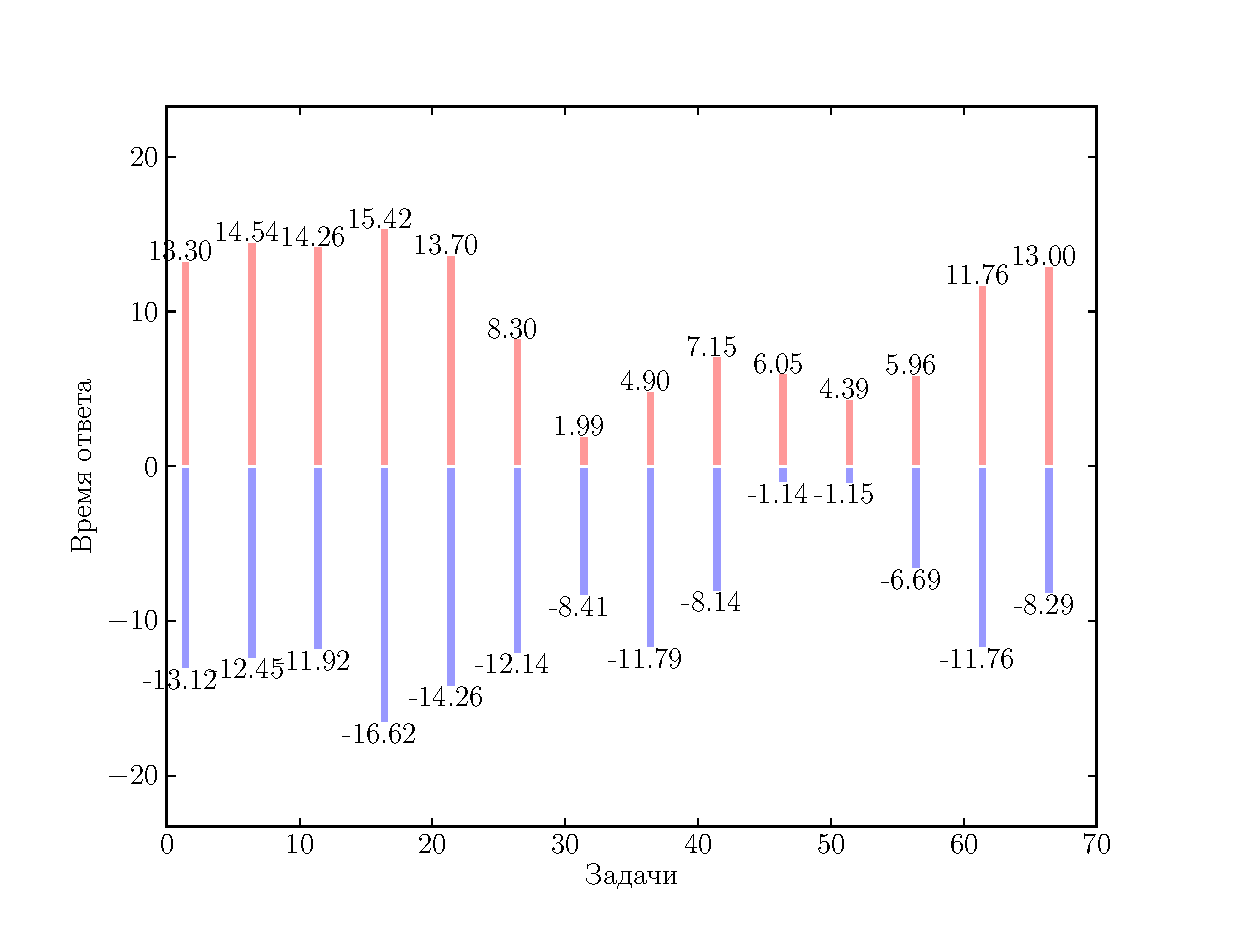
\includegraphics[scale=0.85]{forecast.eps}
\caption{Сравнение прогнозных и модельных данных}
\end{figure}

\newpage
Построим ещё одну диаграмму, на которой отобразим разность между смоделированными и прогнозными данными - ошибку прогноза.

\begin{figure}[ht!]
\centering 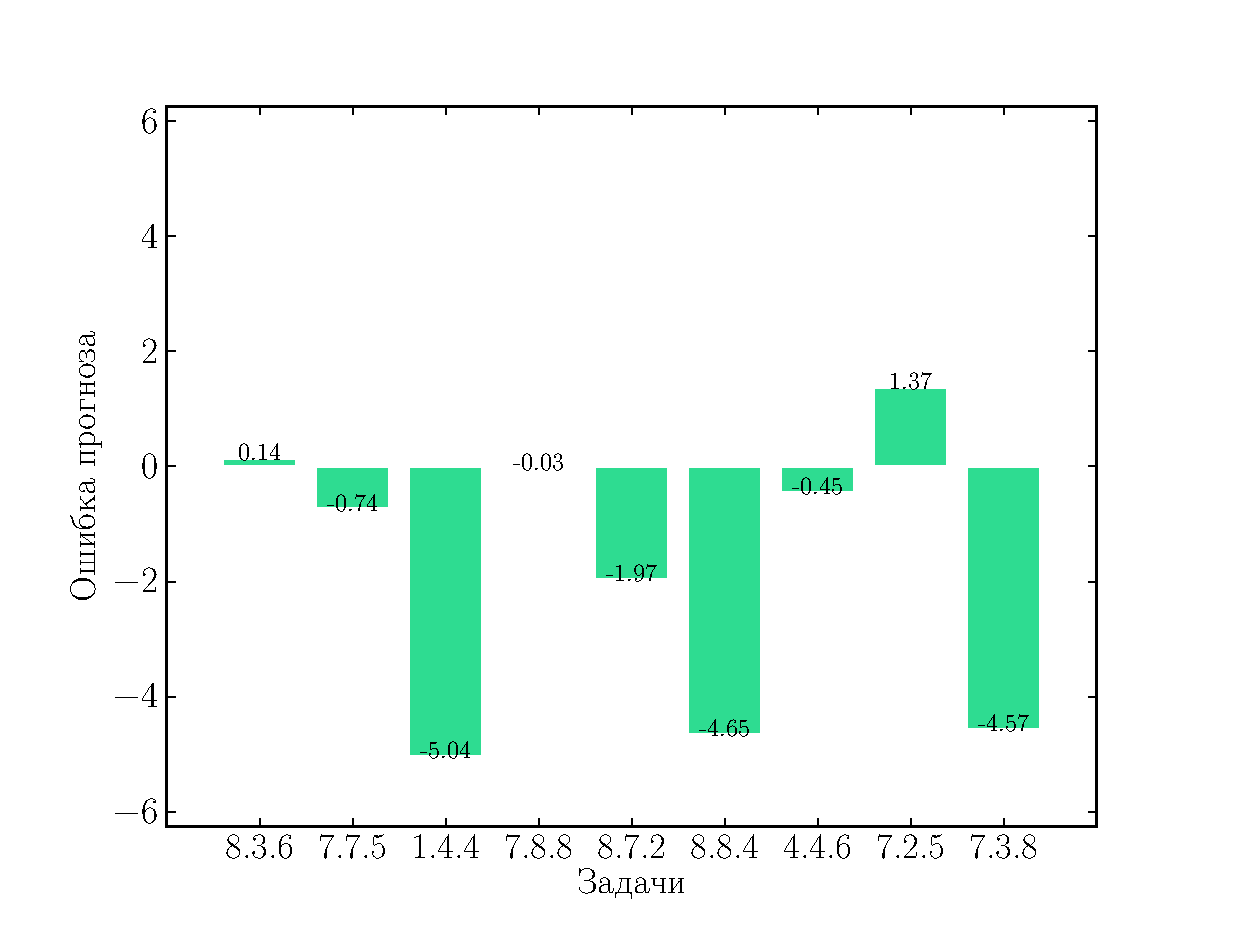
\includegraphics[scale=0.85]{fdiffer.eps}
\caption{Ошибка прогноза}
\end{figure}
На диаграмме видно, что ошибка прогноза для <<скомпроментированных>> задач выше, чем для задач, которые решались честно - фактическое время ответа на такие задачи значительно меньше, чем прогнозное. Используем эту идею для выяв\-ления <<скомпроментированных>> задач.

Алгоритм выявления скомпроментированных задач:
\begin{enumerate}
\item на основании имеющейся информации получить оценки для параметров $\hat{\mu}, \hat{\tau_j}, \hat{\beta_i}, \hat{\sigma}_{ij}$;
\item для студента $j$ при ответе на задачу $i$ вычисляем параметры распре\-деления времени ответа: $\log T_{ij}\sim N_{ij}(\hat{\mu}+\hat{\tau_j}+\hat{\beta_i}, \hat{\sigma}^{2}_{ij})$;
\item находим левую границу одностороннего интервала на уровне довери\-тельной вероятности $p=0.05$ (квантиль уровня $p$\cite{23.});
\item если время ответа меньше полученной левой границы - задачу считаем скомпроментированной;
\end{enumerate}

Описанная модель позволяет решить две основных задачи: во-первых, выявить студентов, которые пользуются готовыми ответами при работе с СДО, а во-вторых, выяснить скомпроментированные задачи и удалить их из пула заданий для данной группы студентов. 